\section{Mechanik}

\subsection{Mechanische Struktur}
Das Grundgerüst des Beercoolers besteht aus 2 MDF-Holzplatten, welche über Stützen miteinander verschraubt werden, sodass zwischen ihnen ein Hohlraum entsteht. In diesem Hohlraum ist Platz für sämtliche Elektronik, wie den  Motoren, den Mikrokontroller und dem Akku. Auf der Rückseite des Roboters befindet sich an der oberen Platte ein Rad mit neutraler Lenkung, am vorderen Ende befinden sich zwei angetriebene Räder.  Zuerst war geplant mit 4 starren angetriebenen Rädern zu fahren. Da dieses System aber im beladenen Zustand schlecht lenkbar war, haben wir uns für die Lösung mit einem neutralen Lenkrad entschieden.\\
\\
Auf der oberen Platte befinden sich 4 Führungen, in welchen die Kühlbox zu platzieren ist. Die elektrische Verbindung ist in die Platte eingearbeitet und stellt eine einwandfreie Verbindung sicher. Die Kühlbox lässt sich dann auf Heizen oder Kühlen einstellen.

\begin{figure}[H]
    \begin{center}
    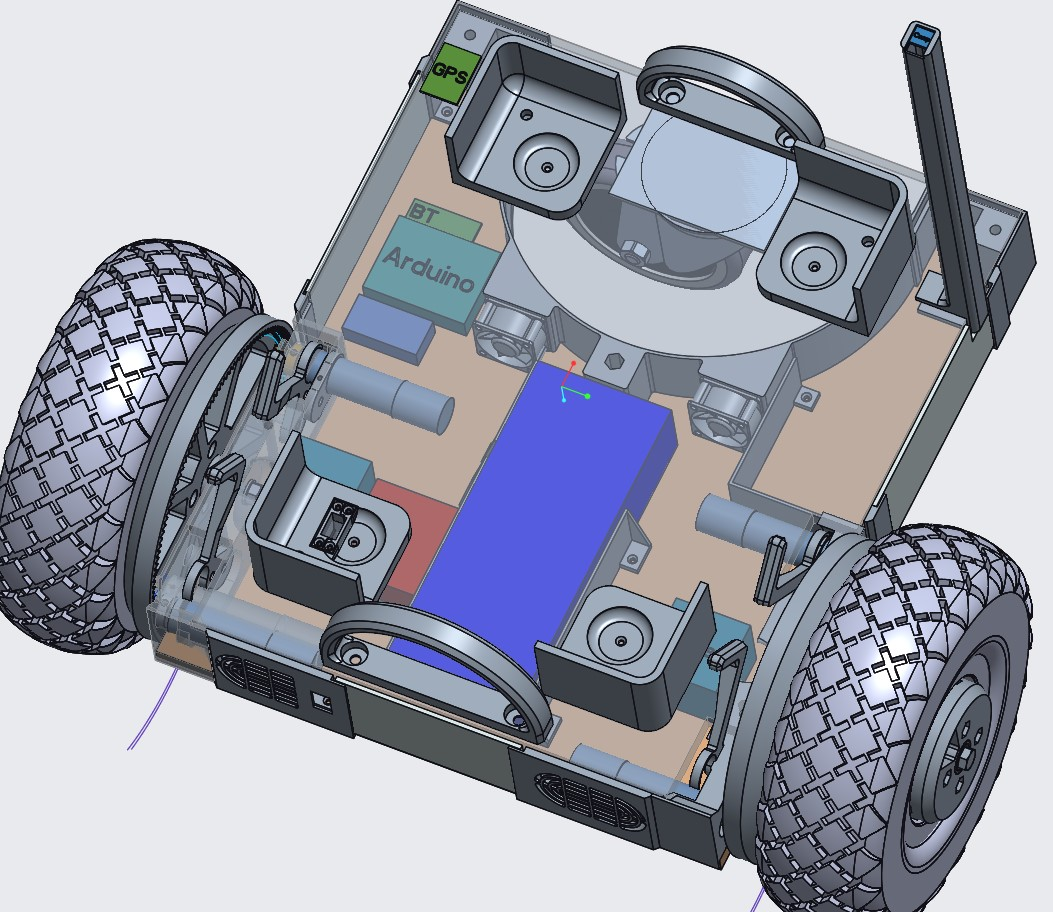
\includegraphics[width=8cm]{Aufbau.jpg}
    \end{center}
    \caption{Aufbau im CAD}
\end{figure}

\subsection{Führungen / Getriebe}
Die Fortbewegung wird über 4 Brushless DC-Motoren von Faulhaber und ein Zahnradpaar gewährleistet. Der Kraftschluss geschieht über ein direkt auf der Motorwelle montiertes kleines, und über ein innenverzahntes grosses Zahnrad, welches mit dem Rad verschraubt ist.\\

\begin{figure}[H]
    \begin{center}
    \includegraphics[width=6cm]{Führungen Getriebe_Zahnrad.jpg}
    \end{center}
    \caption{3D gedruckte Zahnräder}
\end{figure}

Die Motoren sind zudem über einen Hebelmechanismus zurückziehbar, wodurch es möglich ist den Roboter auch ohne den Einsatz der Motoren so reibungsfrei wie möglich zu bewegen. 

\begin{figure}[H]
    \begin{center}
    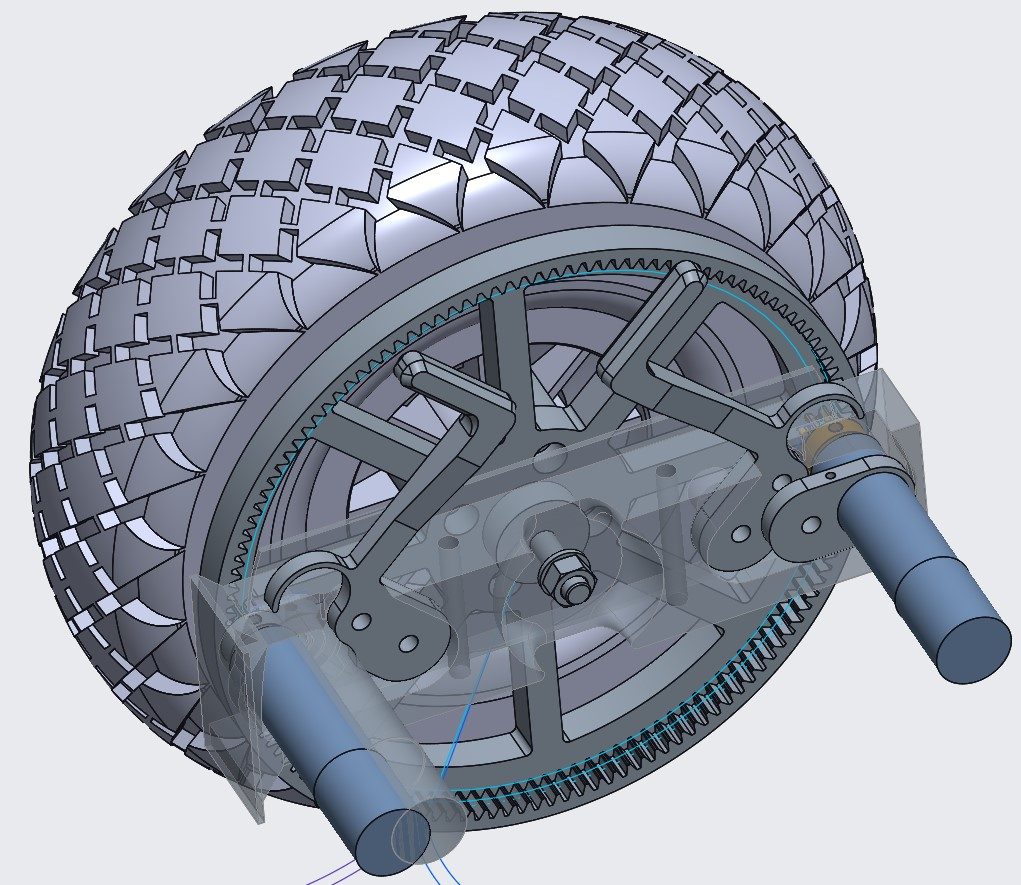
\includegraphics[width=6cm]{rad_asm.jpg}
    \end{center}
    \caption{Rad mit Aufnahme und Hebelmechanismus}
\end{figure}

Um eine reibungsfreie Bewegung zu Erreichen, wurden bei den angetriebenen Rädern Kugellager eingebaut. Hier ist es wichtig, auf den korrekten Einbau der Kugellager zu achten, damit durch den Zusammenbau der Baugruppe keine überhöhten axiale Kräfte auf das Lager wirken. Dies kann zum Versagen der Lager führen.  Weil wir zu Beginn die Lager nicht richtig abgestützt haben, hat sich ein Kugellager während den Testversuchen in Einzelteile zerlegt. Dieses Problem konnte mit einer Hülse, welche die Innenringe der Kugellager abstützt, gelöst werden, so dass keine axiale Last durch das Anziehen der Schraube auf den Kugellagern lastet.